%!TEX root = CooperBarba2014.tex

The implicit-solvent model uses continuum electrostatics to describe the mean-field potential in a molecular system. A typical system consists of a protein in a solvent, defining two regions: inside and outside the protein, with an interface marked by the solvent-excluded surface (\ses).  The \ses, beyond which a water molecule cannot penetrate into the protein, can be generated by rolling a (virtual) spherical probe of the size of a water molecule around the protein (see Figure \ref{fig:forcefield-ses}). Inside the protein, the domain has low permittivity ($\epsilon= 2\text{ to }4$) and there are point charges located at the positions of the atoms. The solvent region, representing water with salt, has a permittivity of $\epsilon \approx 80$. A system of partial differential equations models this situation, with a Poisson equation governing inside the protein and a linearized Poisson-Boltzmann equation governing in the solvent region. Appropriate interface conditions on the \ses express the continuity of the potential and electric displacement, completing the mathematical formulation.

\begin{figure}% [h]
   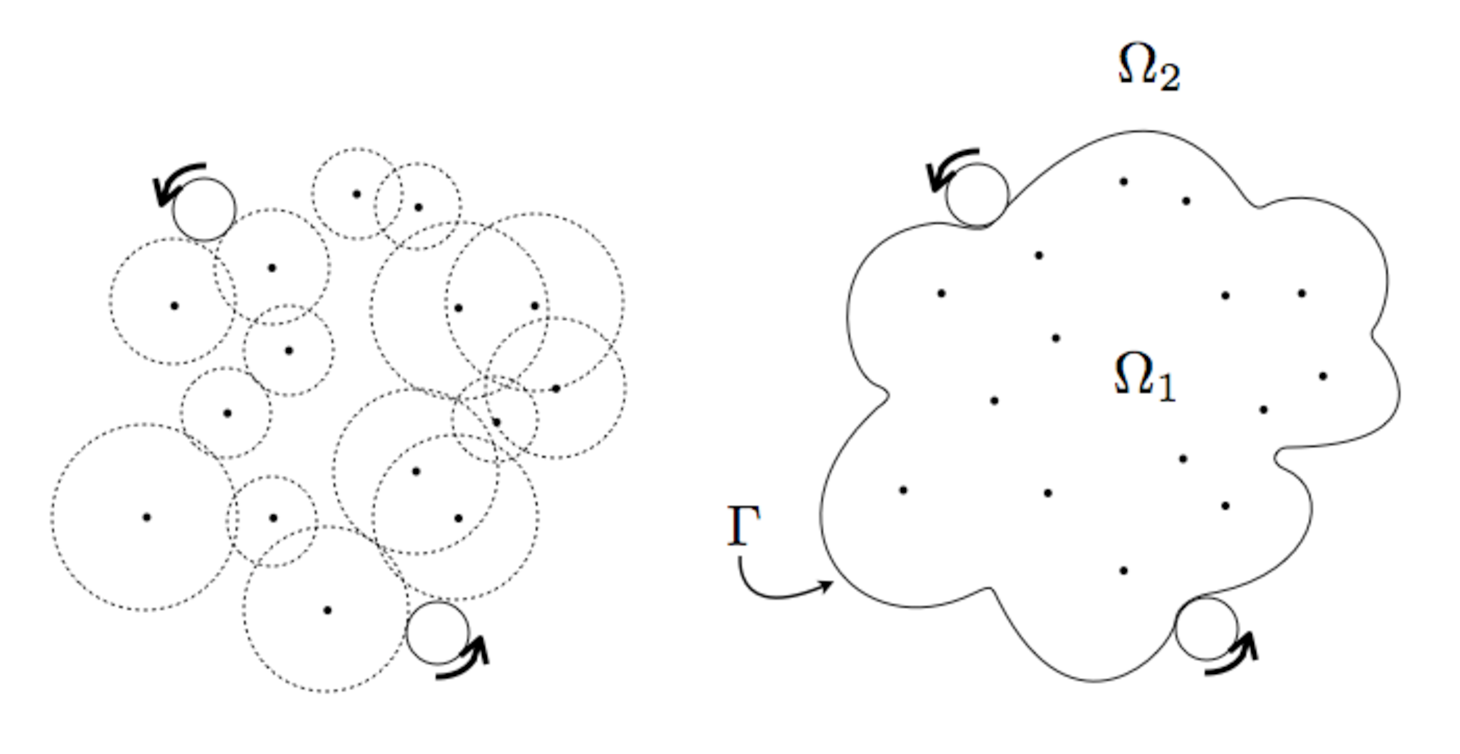
\includegraphics[width=0.49\textwidth]{Figure1.pdf} 
   \caption{Sketch of the process for generating a solvent-excluded surface (\ses): a protein molecule contains a set of atoms that define a radius upon applying a force field and a probe the size of a water molecule is rolled to define the  \ses. $\Omega_1$ is the protein region and $\Omega_2$ the solvent region.}
   \label{fig:forcefield-ses}
\end{figure}

This model has been widely applied to investigate interactions between molecules, such as in protein-ligand binding. We are interested here in an extension of the model to consider interactions between  proteins and surfaces with an imposed potential or charge. This new setup is sketched in Figure \ref{fig:molecule_surface}, and is described mathematically by the following equations:


\begin{align} \label{eq:pde}
\nabla^2 \phi_1(\mathbf{r}) &= - \sum_k \frac{q_k}{\epsilon_1} \delta(\mathbf{r},\mathbf{r}_k) \ \text{ in solute $(\Omega_1)$,}  \nonumber \\ 
\nabla^2\phi_2 (\mathbf{r}) &= \kappa^2 \phi_2(\mathbf{r}) \quad \qquad \ \ \text{ in solvent $(\Omega_2)$,}  \nonumber \\ 
\phi_1 &=\phi_2 \qquad \qquad \qquad \text{ on interface $\Gamma_1$,}  \nonumber \\ 
\epsilon_1 \frac{\partial \phi_1}{\partial \mathbf{n}} &= \epsilon_2 \frac{\partial \phi_2}{\partial \mathbf{n}} \nonumber \\
\phi_2 = \phi_0 &\text{ or } -\epsilon_2 \frac{\partial \phi_2}{\partial \mathbf{n}} = \sigma_0 \ \ \text{ on surface $\Gamma_2$,} 
\end{align}

\noindent Here, $\phi_i$ is the potential corresponding to the region $\Omega_i$ with permittivity $\epsilon_i$, and $\phi_0$ and $\sigma_0$ are the set potential or charge on the nanosurface. 

\begin{figure}
   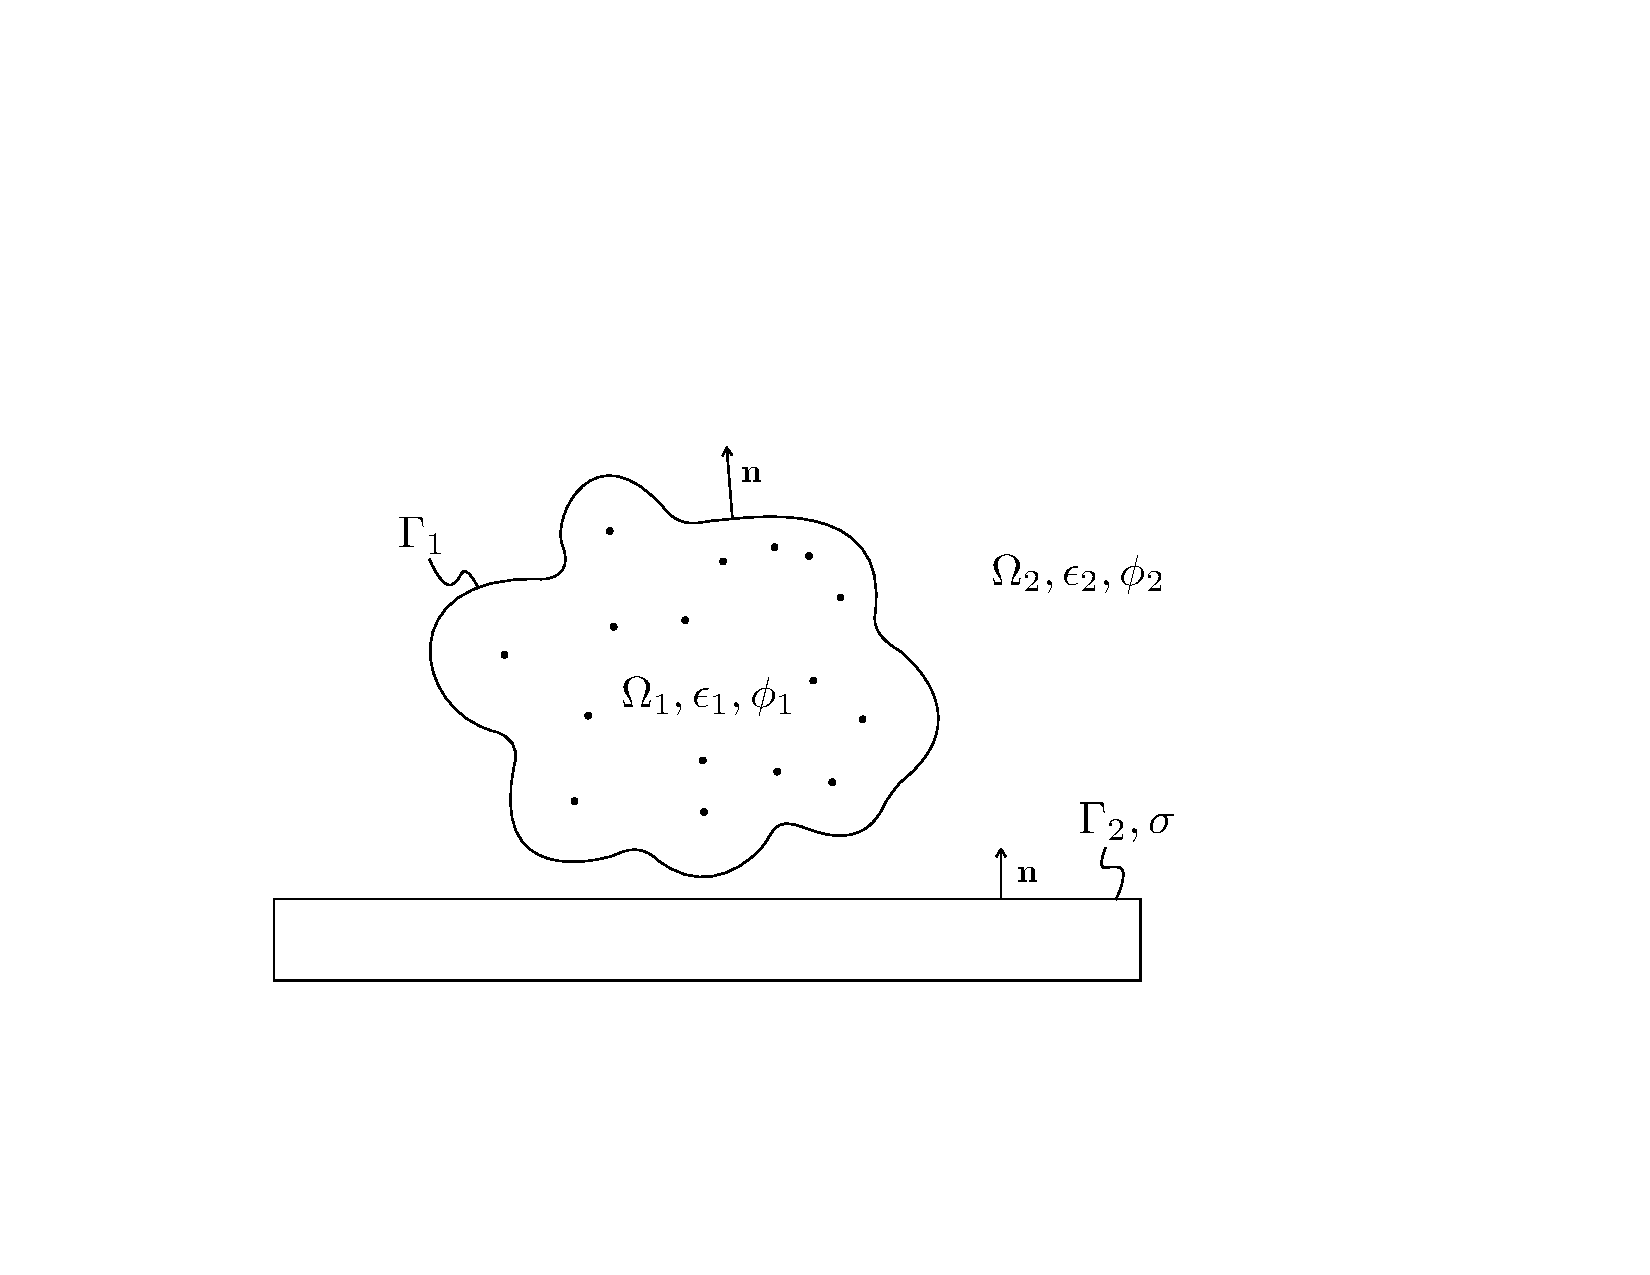
\includegraphics[width=0.45\textwidth]{Figure2.pdf} 
   \caption{Sketch of a molecule interacting with a surface: $\Omega_1$ is the protein, $\Omega_2$ the solvent region, $\Gamma_1$ is the  \ses and $\Gamma_2$ a nanosurface with imposed charge or potential.}
   \label{fig:molecule_surface}
\end{figure}
